\documentclass[tikz]{standalone}

\begin{document}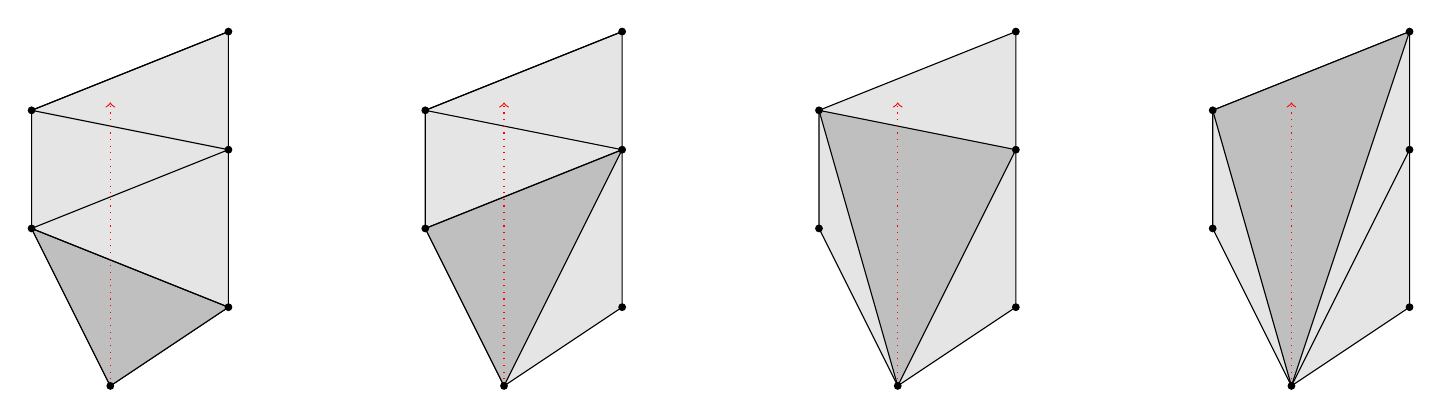
\begin{tikzpicture}

\coordinate (b) at (-.5,0);
\coordinate (l0) at (-1.5,2);
\coordinate (l1) at (-1.5,3.5);
\coordinate (r0) at (1,1);
\coordinate (r1) at (1,3);
\coordinate (r2) at (1,4.5);
\coordinate (t) at (0.5,6);

\filldraw[draw=black,fill=gray!20] (b) -- (l0) -- (l1) -- (r2) -- (r0) -- (b) -- cycle;




\filldraw[draw=black,fill=gray!50] (b) -- (l0) -- (r0) -- cycle;

\draw (l0) -- (r0);
\draw (l0) -- (r1);
\draw (l1) -- (r1);
\draw (l1) -- (r2);

\draw[red,dotted,->] (b) -- +(0,3.6);

\node[circle,fill=black,inner sep=1pt] at (b) {};
\node[circle,fill=black,inner sep=1pt] at (l0) {};
\node[circle,fill=black,inner sep=1pt] at (l1) {};
\node[circle,fill=black,inner sep=1pt] at (r0) {};
\node[circle,fill=black,inner sep=1pt] at (r1) {};
\node[circle,fill=black,inner sep=1pt] at (r2) {};








\begin{scope}[xshift=5cm]
\coordinate (b) at (-.5,0);
\coordinate (l0) at (-1.5,2);
\coordinate (l1) at (-1.5,3.5);
\coordinate (r0) at (1,1);
\coordinate (r1) at (1,3);
\coordinate (r2) at (1,4.5);
\coordinate (t) at (0.5,6);

\filldraw[draw=black,fill=gray!20] (b) -- (l0) -- (l1) -- (r2) -- (r0) -- (b) -- cycle;




\filldraw[draw=black,fill=gray!50] (b) -- (l0) -- (r1) -- cycle;

\draw (l0) -- (r1);
\draw (l1) -- (r1);
\draw (l1) -- (r2);

\draw[red,dotted,->] (b) -- +(0,3.6);
\node[circle,fill=black,inner sep=1pt] at (b) {};
\node[circle,fill=black,inner sep=1pt] at (l0) {};
\node[circle,fill=black,inner sep=1pt] at (l1) {};
\node[circle,fill=black,inner sep=1pt] at (r0) {};
\node[circle,fill=black,inner sep=1pt] at (r1) {};
\node[circle,fill=black,inner sep=1pt] at (r2) {};







\end{scope}

\begin{scope}[xshift=10cm]
\coordinate (b) at (-.5,0);
\coordinate (l0) at (-1.5,2);
\coordinate (l1) at (-1.5,3.5);
\coordinate (r0) at (1,1);
\coordinate (r1) at (1,3);
\coordinate (r2) at (1,4.5);
\coordinate (t) at (0.5,6);

\filldraw[draw=black,fill=gray!20] (b) -- (l0) -- (l1) -- (r2) -- (r0) -- (b) -- cycle;




\filldraw[draw=black,fill=gray!50] (b) -- (l1) -- (r1) -- cycle;

\draw[red,dotted,->] (b) -- +(0,3.6);

\node[circle,fill=black,inner sep=1pt] at (b) {};
\node[circle,fill=black,inner sep=1pt] at (l0) {};
\node[circle,fill=black,inner sep=1pt] at (l1) {};
\node[circle,fill=black,inner sep=1pt] at (r0) {};
\node[circle,fill=black,inner sep=1pt] at (r1) {};
\node[circle,fill=black,inner sep=1pt] at (r2) {};







\end{scope}

\begin{scope}[xshift=15cm]
\coordinate (b) at (-.5,0);
\coordinate (l0) at (-1.5,2);
\coordinate (l1) at (-1.5,3.5);
\coordinate (r0) at (1,1);
\coordinate (r1) at (1,3);
\coordinate (r2) at (1,4.5);
\coordinate (t) at (0.5,6);

\filldraw[draw=black,fill=gray!20] (b) -- (l0) -- (l1) -- (r2) -- (r0) -- (b) -- cycle;




\filldraw[draw=black,fill=gray!50] (b) -- (l1) -- (r2) -- cycle;

\draw[red,dotted,->] (b) -- +(0,3.6);

\draw (b) -- (r1);
\node[circle,fill=black,inner sep=1pt] at (b) {};
\node[circle,fill=black,inner sep=1pt] at (l0) {};
\node[circle,fill=black,inner sep=1pt] at (l1) {};
\node[circle,fill=black,inner sep=1pt] at (r0) {};
\node[circle,fill=black,inner sep=1pt] at (r1) {};
\node[circle,fill=black,inner sep=1pt] at (r2) {};







\end{scope}
\end{tikzpicture}\end{document}
